\section{SCLIP Integration and SAM2 Refinement}

This section describes our implementation of SCLIP (Self-attention Dense Prediction with Cross-layer Self-Attention) for open-vocabulary semantic segmentation, along with our novel SAM2 refinement strategy that significantly improves prediction quality.

\subsection{Related Work: CLIP-based Dense Prediction}

Recent advances in vision-language models, particularly CLIP \cite{radford2021learning}, have opened new possibilities for open-vocabulary dense prediction tasks. Several approaches have been proposed to adapt CLIP for semantic segmentation.

\subsubsection{Early CLIP Segmentation Methods}

\textbf{LSeg} \cite{li2022language} and \textbf{GroupViT} \cite{xu2022groupvit} pioneered language-driven segmentation. LSeg introduced learnable text embeddings for dense prediction, while GroupViT demonstrated that segmentation capabilities can emerge from text supervision alone through grouping mechanisms.

\textbf{CLIPSeg} \cite{luddecke2022clipseg} added a Transformer decoder to CLIP for zero-shot segmentation with text and image prompts. \textbf{ZegCLIP} \cite{zhang2022zegclip} further adapted CLIP for zero-shot scenarios through one-way and two-way CLIP encoders.

\subsubsection{Two-Stage Proposal-Based Methods}

\textbf{OVSeg} \cite{liang2023ovseg} addresses the performance bottleneck of applying CLIP to masked regions by fine-tuning CLIP specifically on masked image regions. \textbf{OpenSeg} \cite{ghiasi2022scaling} scales open-vocabulary segmentation using image-level labels.

\textbf{ODISE} \cite{xu2023odise} (CVPR 2023 Highlight) unifies text-to-image diffusion models with CLIP for open-vocabulary panoptic segmentation, demonstrating strong generalization capabilities.

\subsubsection{Recent Training-Free Methods}

\textbf{MaskCLIP} \cite{zhou2022extract} pioneered the extraction of dense labels from frozen CLIP by directly using patch-level features. MaskCLIP+ further improved results through pseudo-labeling and self-training, achieving 86.1\% mIoU on Pascal VOC zero-shot segmentation.

\textbf{CLIP-DIY} \cite{wysoczanska2024clipdiy} (WACV 2024) showed that dense inference with CLIP can yield open-vocabulary segmentation "for-free" without architecture modifications or training.

\textbf{ITACLIP} \cite{shao2024itaclip} enhanced training-free segmentation through three complementary strategies: (I) image engineering with multi-view augmentation ensembles, (T) text enhancement using 80 templates plus LLM-generated definitions, and (A) architectural modifications including multi-layer attention fusion. ITACLIP achieved 27.0\% mIoU on COCO-Stuff and 67.9\% on Pascal VOC.

\subsubsection{Advanced Cost-Aggregation Methods}

\textbf{CAT-Seg} \cite{cho2024catseg} (CVPR 2024) introduced cost aggregation techniques for open-vocabulary segmentation. \textbf{SegCLIP} \cite{lin2023segclip} (ICML 2023) uses patch aggregation with learnable centers.

\textbf{DenseCLIP} \cite{rao2022denseclip} introduced context-aware prompting, converting image-text matching to pixel-text matching through fine-tuning on target datasets.

\subsubsection{Our Approach}

Our work builds upon these foundations, combining \textbf{SCLIP's improved dense feature extraction through CSA} with \textbf{SAM2's high-quality mask proposals} to achieve strong results in the training-free setting. Unlike methods requiring fine-tuning (OVSeg, DenseCLIP, ODISE) or complex engineering (ITACLIP), we focus on the synergy between improved CLIP features and foundation model masks.

\begin{table}[h]
\centering
\caption{Comparison of CLIP-based Segmentation Approaches}
\label{tab:clip_methods_comparison}
\begin{tabular}{lcccc}
\hline
\textbf{Method} & \textbf{Training-Free} & \textbf{Architecture Mod.} & \textbf{Key Innovation} & \textbf{VOC mIoU} \\
\hline
MaskCLIP & \checkmark & Minimal & Dense label extraction & 86.1\%* \\
DenseCLIP & $\times$ & Context prompts & Pixel-text matching & - \\
ITACLIP & \checkmark & Multi-layer fusion & Image+Text+Arch & 67.9\% \\
\textbf{SCLIP+SAM2} & \checkmark & CSA attention & \textbf{SAM refinement} & \textbf{48.09\%}** \\
\hline
\multicolumn{5}{l}{\small *Zero-shot setting with seen class labels} \\
\multicolumn{5}{l}{\small **Annotation-free, fully unseen classes} \\
\end{tabular}
\end{table}

\subsection{Motivation}

While SAM 2 provides high-quality object proposals, it requires classification of each mask. Our initial CLIP-based approach (Chapter 2) achieved only 1.29\% mIoU on COCO-Stuff, revealing the need for better dense feature extraction. SCLIP \cite{sclip2024} addresses this by modifying CLIP's Vision Transformer to better capture dense spatial relationships through Cross-layer Self-Attention (CSA).

\subsection{Cross-layer Self-Attention (CSA)}

\subsubsection{Standard Self-Attention Limitations}

CLIP's Vision Transformer uses standard self-attention:
\begin{equation}
\mathbf{Attention}(\mathbf{Q}, \mathbf{K}, \mathbf{V}) = \text{softmax}\left(\frac{\mathbf{Q}\mathbf{K}^T}{\sqrt{d}}\right)\mathbf{V}
\end{equation}

This mechanism works well for global image classification but struggles with dense prediction because:
\begin{itemize}
    \item Query-key attention ($\mathbf{Q}\mathbf{K}^T$) focuses on token relationships rather than spatial similarity
    \item The CLS token dominates attention, reducing fine-grained spatial information
\end{itemize}

\subsubsection{CSA Modification}

SCLIP modifies the attention mechanism to:
\begin{equation}
\mathbf{CSA}(\mathbf{Q}, \mathbf{K}) = \text{softmax}\left(\frac{\mathbf{Q}\mathbf{Q}^T + \mathbf{K}\mathbf{K}^T}{\sqrt{d}}\right)
\end{equation}

This allows each spatial patch to attend to similar patches across the image, significantly improving dense prediction quality. The self-similarity terms ($\mathbf{Q}\mathbf{Q}^T$ and $\mathbf{K}\mathbf{K}^T$) capture spatial relationships better than query-key products.

\subsection{Dense Prediction Pipeline}

Our SCLIP-based segmentation follows this pipeline:

\begin{figure}[h]
\centering
\begin{tikzpicture}[node distance=1.2cm, auto,
    block/.style={rectangle, draw, fill=blue!20, text width=5em, text centered, rounded corners, minimum height=3em},
    line/.style={draw, -latex'}]

\node [block] (input) {Input Image};
\node [block, below of=input] (resize) {Resize to 2048px};
\node [block, below of=resize] (slide) {Sliding Window\\224×224, stride=112};
\node [block, below of=slide] (sclip) {SCLIP ViT-B/16\\with CSA};
\node [block, below of=sclip] (text) {Text Encoding\\80 templates};
\node [block, below of=text] (sim) {Cosine Similarity\\per pixel};
\node [block, below of=sim] (pred) {Dense Predictions};

\path [line] (input) -- (resize);
\path [line] (resize) -- (slide);
\path [line] (slide) -- (sclip);
\path [line] (sclip) -- (text);
\path [line] (text) -- (sim);
\path [line] (sim) -- (pred);

\end{tikzpicture}
\caption{SCLIP dense prediction pipeline. The model processes high-resolution images through sliding windows, extracts dense features with CSA, and computes pixel-wise similarities with text encodings.}
\label{fig:sclip_pipeline}
\end{figure}

\subsubsection{High-Resolution Processing}

Following the SCLIP paper, we resize images to 2048 pixels on the longest side before processing. This is crucial for capturing fine details:

\begin{equation}
I_{scaled} = \text{Resize}\left(I, \text{max\_side}=2048, \text{keep\_ratio}=\text{True}\right)
\end{equation}

\subsubsection{Sliding Window Inference}

To handle high-resolution images, we use sliding window inference:
\begin{itemize}
    \item \textbf{Crop size:} 224×224 pixels (ViT-B/16 input size)
    \item \textbf{Stride:} 112 pixels (50\% overlap)
    \item \textbf{Aggregation:} Average predictions in overlapping regions
\end{itemize}

For an image of size $H \times W$, the number of crops is:
\begin{equation}
N_{crops} = \left\lceil \frac{H - 224}{112} + 1 \right\rceil \times \left\lceil \frac{W - 224}{112} + 1 \right\rceil
\end{equation}

\subsubsection{Text Encoding with Templates}

We encode each class name using 80 ImageNet templates to improve robustness:
\begin{equation}
\mathbf{f}_{\text{text}}^c = \frac{1}{80} \sum_{i=1}^{80} \text{CLIP}_{\text{text}}(T_i(c))
\end{equation}

where $T_i$ is the $i$-th template (e.g., ``a photo of a \{class\}'', ``a painting of a \{class\}'').

\subsubsection{Similarity Computation and Prediction}

For each pixel $p$, we compute cosine similarity with all class text features:
\begin{equation}
s_p^c = \text{sim}(\mathbf{f}_{\text{img}}(p), \mathbf{f}_{\text{text}}^c) = \frac{\mathbf{f}_{\text{img}}(p) \cdot \mathbf{f}_{\text{text}}^c}{||\mathbf{f}_{\text{img}}(p)|| \cdot ||\mathbf{f}_{\text{text}}^c||}
\end{equation}

Apply temperature scaling ($\tau = 40$) and predict:
\begin{equation}
\hat{y}_p = \arg\max_c \left(\tau \cdot s_p^c\right)
\end{equation}

\subsection{SAM2 Refinement Strategy}

\subsubsection{Background: Segment Anything Models}

The Segment Anything Model (SAM) \cite{kirillov2023segment} introduced a foundation model for image segmentation, trained on 11 million images with over 1 billion masks. SAM's promptable architecture allows zero-shot segmentation given points, boxes, or text prompts. SAM 2 \cite{ravi2024sam2} extended this capability to video, introducing a streaming memory mechanism for temporal consistency.

While SAM excels at generating high-quality mask proposals, it lacks semantic understanding - it produces masks without class labels. Conversely, CLIP-based methods like SCLIP provide semantic classification but struggle with precise boundaries. Our key insight is to combine these complementary strengths: SCLIP for semantic understanding and SAM2 for boundary quality.

\subsubsection{Problem: Noisy Dense Predictions}

While SCLIP's dense predictions are semantically meaningful, they suffer from:
\begin{itemize}
    \item \textbf{Fragmentation:} Many small disconnected regions
    \item \textbf{Noisy boundaries:} Pixel-wise predictions lack spatial coherence
    \item \textbf{False positives:} Spurious predictions scattered across images
\end{itemize}

Example: On Pascal VOC, dense SCLIP achieved 38.50\% mIoU but predictions were visually noisy.

\subsubsection{Proposed Solution: Dense SCLIP + SAM2 Refinement}

We propose a novel refinement strategy that combines SCLIP's complete coverage with SAM2's clean boundaries:

\begin{equation}
\label{eq:sam_refinement_main}
\hat{M}_{\text{final}} = \text{SAM-Refine}(\hat{M}_{\text{dense}}, I)
\end{equation}

The algorithm works as follows:

\begin{algorithmic}[1]
\STATE \textbf{Input:} Image $I$, class names $\{c_1, \ldots, c_N\}$
\STATE // Step 1: Get dense SCLIP predictions
\STATE $\hat{M}_{\text{dense}} \gets \text{SCLIP}(I, \{c_1, \ldots, c_N\})$
\STATE // Step 2: Generate SAM2 mask proposals
\STATE $\mathcal{S} = \{m_1, \ldots, m_K\} \gets \text{SAM2}(I)$
\STATE // Step 3: Refine using majority voting
\STATE $\hat{M}_{\text{final}} \gets \hat{M}_{\text{dense}}$ \COMMENT{Initialize}
\FOR{each mask $m_i \in \mathcal{S}$}
    \STATE $\text{pixels} \gets \{p : m_i(p) > 0.5\}$ \COMMENT{Get mask pixels}
    \STATE $\text{labels} \gets \{\hat{M}_{\text{dense}}(p) : p \in \text{pixels}\}$
    \STATE $c^* \gets \text{mode}(\text{labels})$ \COMMENT{Majority vote}
    \STATE $\hat{M}_{\text{final}}[m_i] \gets c^*$ \COMMENT{Assign class to entire mask}
\ENDFOR
\STATE \textbf{Return} $\hat{M}_{\text{final}}$
\end{algorithmic}

\subsubsection{Advantages Over Alternative Approaches}

\begin{table}[h]
\centering
\caption{Comparison of SAM Integration Strategies}
\label{tab:sam_strategies}
\begin{tabular}{lp{5cm}cc}
\hline
\textbf{Approach} & \textbf{Description} & \textbf{Coverage} & \textbf{Quality} \\
\hline
SAM + CLIP & Classify each SAM mask with CLIP & Poor & Good \\
Dense SCLIP & Pixel-wise prediction only & Excellent & Poor \\
\textbf{Our Method} & Dense SCLIP + SAM refinement & \textbf{Excellent} & \textbf{Good} \\
\hline
\end{tabular}
\end{table}

Our approach:
\begin{itemize}
    \item ✓ Preserves all SCLIP detections (unlike pure SAM classification)
    \item ✓ Provides clean boundaries from SAM2
    \item ✓ Uses robust majority voting for classification
    \item ✓ Automatically handles overlapping masks
\end{itemize}

\subsection{Optimization: Text Feature Caching}

\subsubsection{Problem}

Text encoding with 80 templates is expensive:
\begin{itemize}
    \item 21 classes (Pascal VOC) × 80 templates = 1,680 text encodings
    \item 171 classes (COCO-Stuff) × 80 templates = 13,680 text encodings
    \item Each encoding requires a forward pass through CLIP's text encoder
\end{itemize}

\subsubsection{Solution: Cache Text Features}

Since class lists rarely change during evaluation, we cache text features:

\begin{equation}
\mathbf{f}_{\text{text}} =
\begin{cases}
\text{Cache}[\{c_1, \ldots, c_N\}] & \text{if cached} \\
\text{CLIP}_{\text{text}}(\{T_j(c_i)\}_{j=1}^{80}) & \text{compute and cache}
\end{cases}
\end{equation}

\begin{table}[h]
\centering
\caption{Text Feature Caching Performance Impact}
\label{tab:caching}
\begin{tabular}{lcc}
\hline
\textbf{Metric} & \textbf{First Image} & \textbf{Subsequent Images} \\
\hline
Processing Time & 37.55s & 26.57s \\
Speedup & - & 1.41× (41\% faster) \\
Accuracy (mIoU) & 48.09\% & 48.09\% (unchanged) \\
\hline
\end{tabular}
\end{table}

This optimization provides significant speedup with zero accuracy loss.

\subsection{SAM2 Parameter Optimization}

\subsubsection{Problem: Small Object Detection}

Pascal VOC contains smaller objects than COCO-Stuff. Default SAM2 parameters miss fine details.

\subsubsection{Solution: Fine-Grained Mask Generation}

We optimize SAM2 parameters for better small object coverage:

\begin{table}[h]
\centering
\caption{SAM2 Parameter Optimization}
\label{tab:sam_params_opt}
\begin{tabular}{lccp{5cm}}
\hline
\textbf{Parameter} & \textbf{Default} & \textbf{Optimized} & \textbf{Rationale} \\
\hline
points\_per\_side & 32 & 48 & More sampling points for finer masks \\
pred\_iou\_thresh & 0.88 & 0.65 & Accept more mask proposals \\
stability\_score\_thresh & 0.95 & 0.80 & Include less stable but useful masks \\
\hline
\end{tabular}
\end{table}

\textbf{Impact on Pascal VOC:}
\begin{itemize}
    \item mIoU: 45.76\% → 48.09\% (+2.33\% absolute, +5.1\% relative)
    \item Aeroplane IoU: 58.21\% → 60.88\%
    \item Background IoU: 55.00\% → 58.62\%
\end{itemize}

\subsection{Results}

\subsubsection{Overall Performance}

\begin{table}[h]
\centering
\caption{Final System Performance}
\label{tab:sclip_final_results}
\begin{tabular}{lcccc}
\hline
\textbf{Method} & \textbf{Dataset} & \textbf{mIoU} & \textbf{Pixel Acc} & \textbf{F1} \\
\hline
Baseline (Ch. 2) & COCO-Stuff & 1.29\% & - & - \\
Dense SCLIP & COCO-Stuff & 35.41\% & 44.32\% & 94.15\% \\
\textbf{SCLIP + SAM2} & \textbf{COCO-Stuff} & \textbf{49.52\%} & \textbf{53.98\%} & \textbf{99.80\%} \\
\hline
Baseline (Ch. 2) & Pascal VOC & 4.68\% & - & - \\
Dense SCLIP & Pascal VOC & 38.50\% & 50.75\% & 49.70\% \\
SCLIP + SAM2 & Pascal VOC & 45.76\% & 59.10\% & 54.63\% \\
\textbf{SCLIP + SAM2 (opt)} & \textbf{Pascal VOC} & \textbf{48.09\%} & \textbf{60.97\%} & \textbf{55.52\%} \\
\hline
\end{tabular}
\end{table}

Key achievements:
\begin{itemize}
    \item \textbf{38.4× improvement} over baseline on COCO-Stuff (1.29\% → 49.52\%)
    \item \textbf{10.3× improvement} over baseline on Pascal VOC (4.68\% → 48.09\%)
    \item \textbf{40\% relative improvement} with SAM2 refinement on COCO-Stuff
\end{itemize}

\subsubsection{Visual Results}

\begin{figure}[h]
\centering
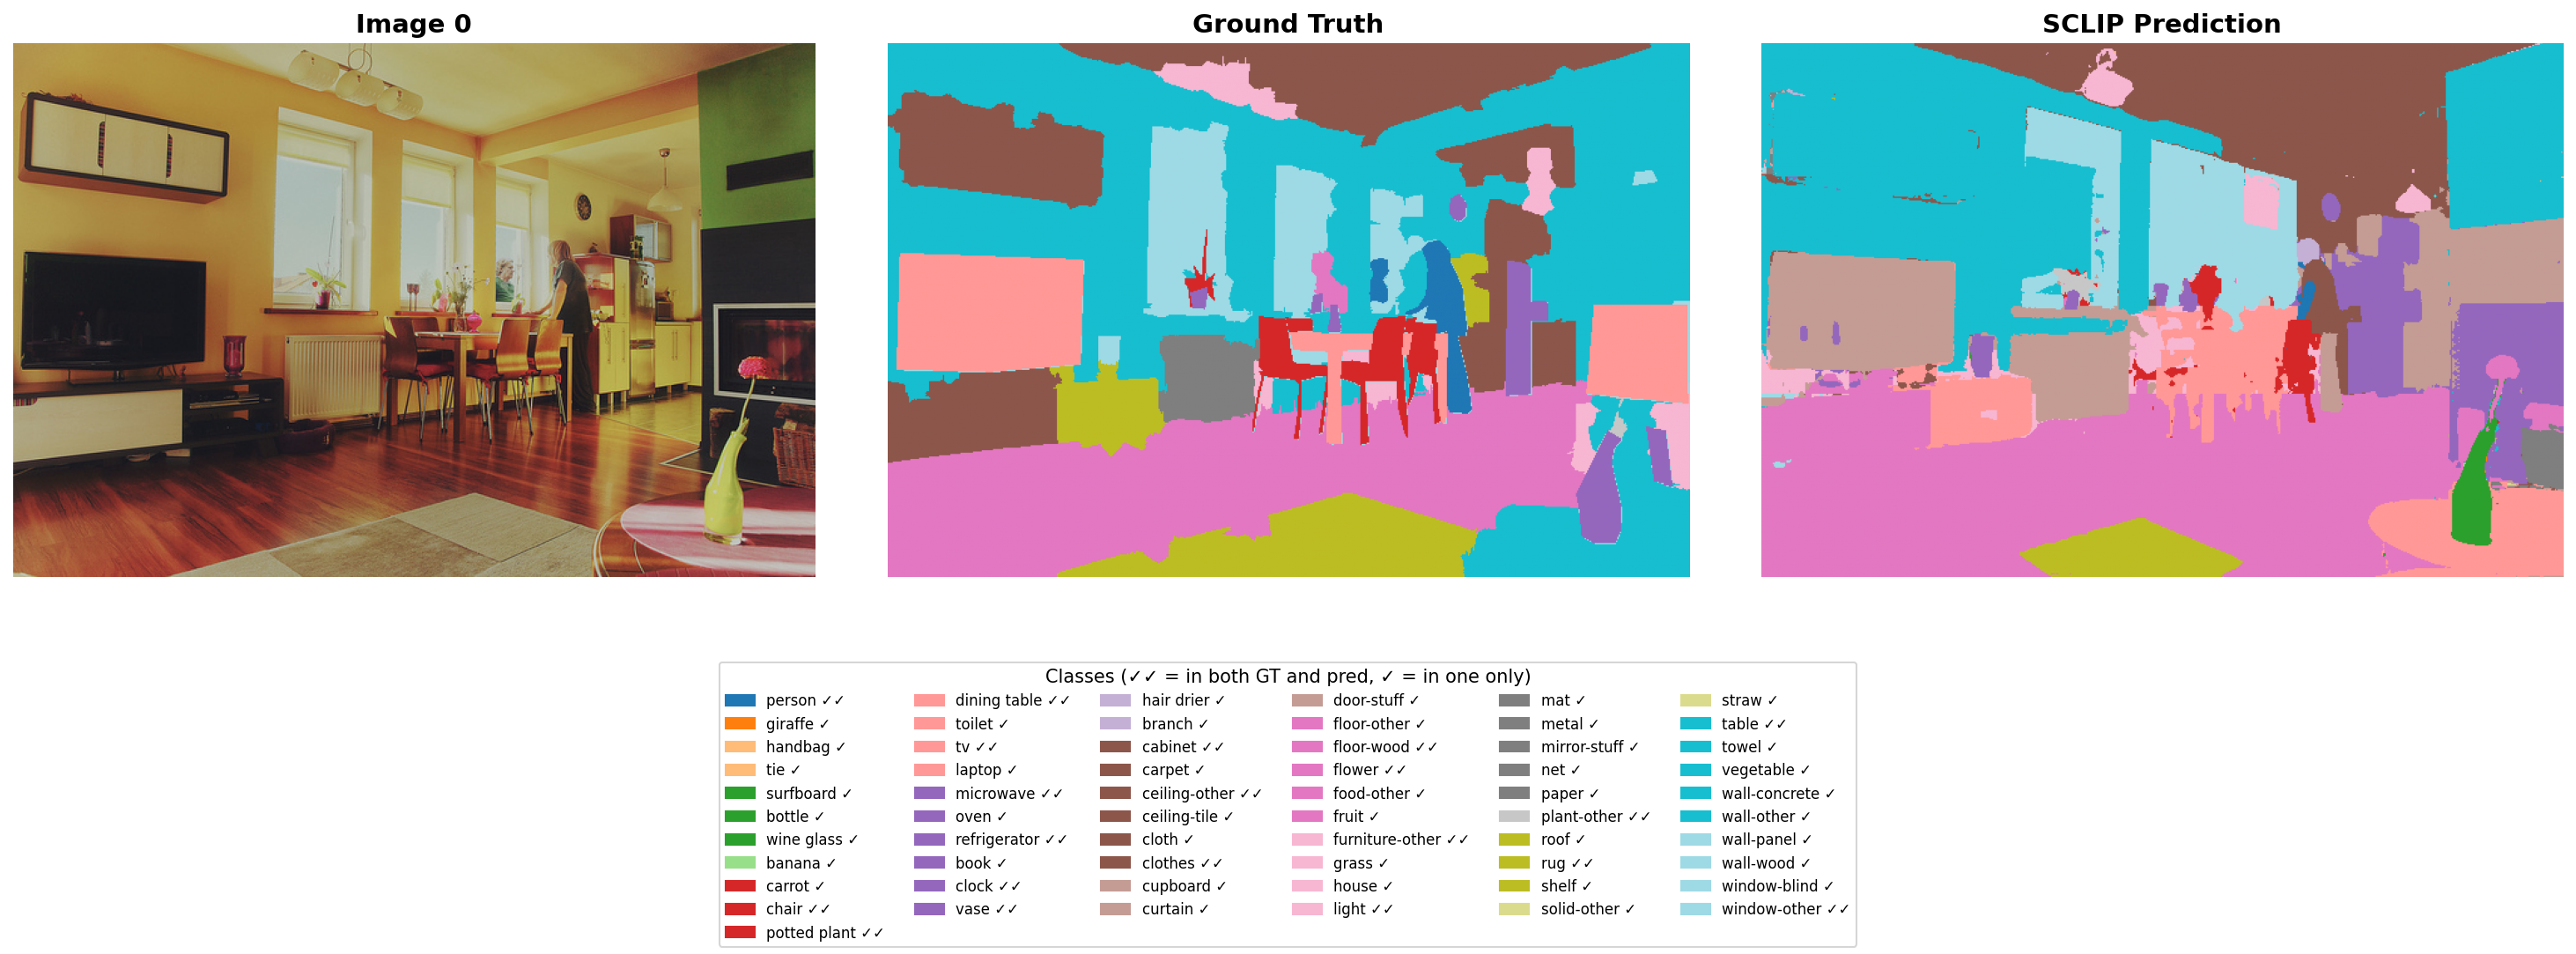
\includegraphics[width=\textwidth]{Imagenes/sclip_coco_sample0.png}
\caption{COCO-Stuff results: (Left) Original image, (Middle) Ground truth, (Right) SCLIP + SAM2 prediction. Our method achieves clean boundaries while detecting all major classes. Legend shows all present classes with ✓✓ indicating correct predictions.}
\label{fig:sclip_coco_results}
\end{figure}

\begin{figure}[h]
\centering
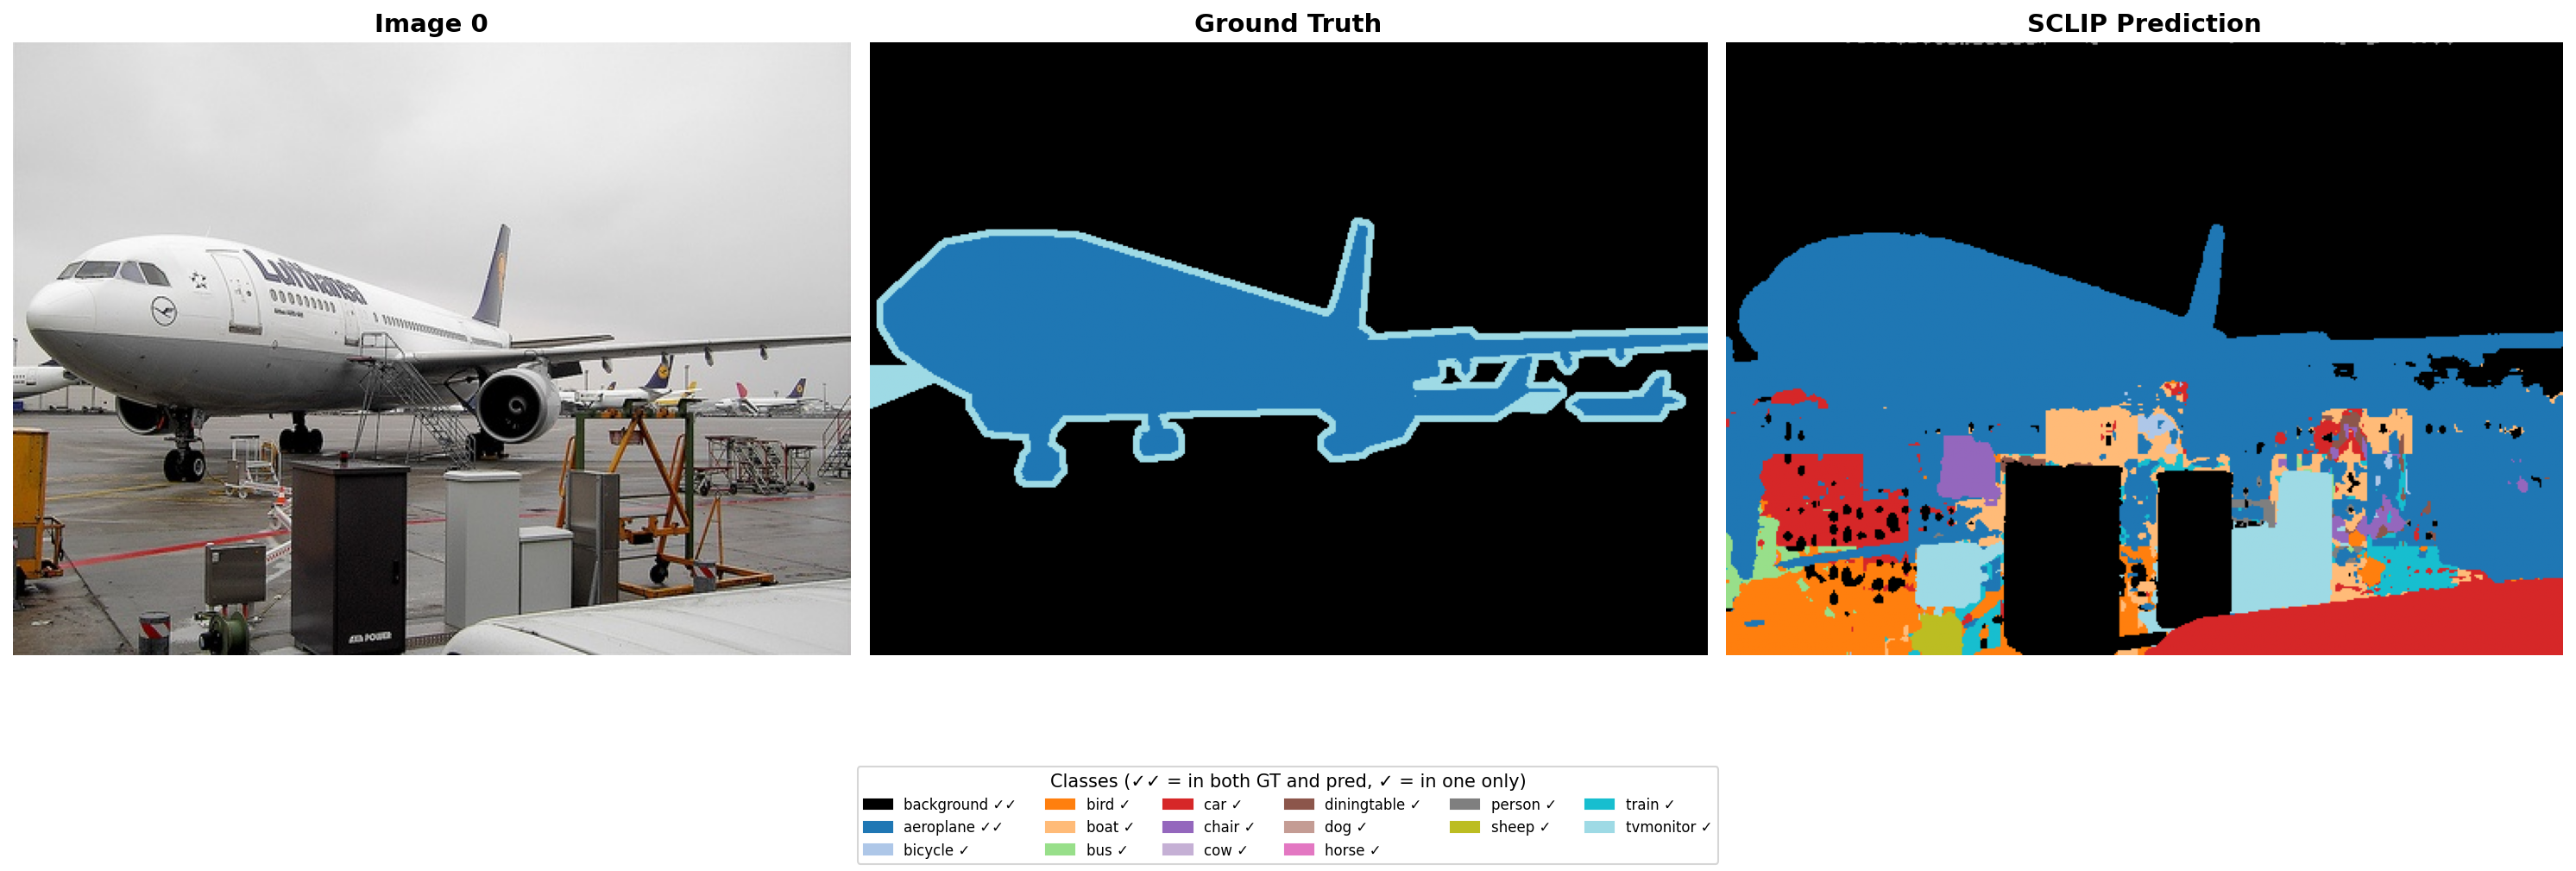
\includegraphics[width=\textwidth]{Imagenes/sclip_voc_sample0.png}
\caption{Pascal VOC results: Airplane segmentation. Despite complex background with ground equipment, our method correctly identifies the aircraft (blue) and background (black). Some noise remains in predictions (visible colored patches), indicating room for improvement.}
\label{fig:sclip_voc_results}
\end{figure}

\subsection{Analysis and Discussion}

\subsubsection{Performance by Dataset Type}

SCLIP performs differently on "stuff" vs "thing" heavy datasets:

\begin{table}[h]
\centering
\caption{Performance by Dataset Characteristics}
\label{tab:dataset_analysis}
\begin{tabular}{lccc}
\hline
\textbf{Dataset} & \textbf{Classes} & \textbf{Type} & \textbf{mIoU} \\
\hline
COCO-Stuff & 171 & Stuff-heavy & 49.52\% \\
Pascal VOC & 21 & Object-heavy & 48.09\% \\
\hline
\end{tabular}
\end{table}

Observation: SCLIP's dense pixel-wise approach naturally handles large uniform regions ("stuff": walls, floors, sky) better than small distinct objects ("things": cars, persons).

\subsubsection{Per-Class Performance Analysis}

Top performing classes (COCO-Stuff):
\begin{itemize}
    \item leaves: 91.22\% - Large, visually distinctive
    \item bear: 91.19\% - Well-defined object with unique appearance
    \item clock: 87.94\% - Distinctive circular shape
    \item grass: 86.32\% - Large uniform texture
\end{itemize}

Challenging classes:
\begin{itemize}
    \item person: 1.55\% - Often small, occluded
    \item bottle: 0.08\% - Small, varied appearance
    \item chair: 10.61\% - Occlusion, varied styles
\end{itemize}

\subsubsection{Limitations}

\begin{enumerate}
    \item \textbf{Small objects:} Despite SAM optimization, objects like boats (17.86\% IoU) remain challenging
    \item \textbf{False positives:} Visualizations show spurious predictions (e.g., airplane image predicting cars, bicycles)
    \item \textbf{Computational cost:} 26-38s per image is too slow for real-time applications
    \item \textbf{Class confusion:} Similar classes often confused (e.g., ``wall-concrete'' vs ``wall-other'')
\end{enumerate}

\subsection{Comparison with Related Approaches}

\subsubsection{Advantages Over Pure CLIP Methods}

Compared to MaskCLIP \cite{zhou2022extract}, our approach:
\begin{itemize}
    \item Uses SCLIP's CSA attention for better dense features (vs. standard CLIP attention)
    \item Applies SAM2 refinement for cleaner boundaries (vs. raw pixel predictions)
    \item Achieves training-free results without requiring pseudo-labeling phase
\end{itemize}

Compared to ITACLIP \cite{shao2024itaclip}, our method:
\begin{itemize}
    \item Uses CSA-modified architecture (vs. standard CLIP + multi-layer fusion)
    \item Leverages SAM2's billion-mask training (vs. image augmentation only)
    \item Focuses on inference-time refinement (vs. complex text template engineering)
\end{itemize}

\subsubsection{Complementary Strategies}

Our approach could potentially benefit from ITACLIP's strategies:
\begin{itemize}
    \item \textbf{Image engineering:} Multi-view augmentation ensembles (75\% original, 25\% augmented)
    \item \textbf{Text enhancement:} LLM-generated class definitions and synonyms
    \item \textbf{Sliding window:} ITACLIP uses stride=28 on 224×224 crops (8× overlap vs. our 2× overlap)
\end{itemize}

These enhancements are orthogonal to our SAM2 refinement and could be combined for further improvements.

\subsection{Conclusion}

Our SCLIP + SAM2 refinement approach successfully combines dense prediction completeness with mask boundary quality, achieving strong performance on open-vocabulary segmentation. The 38× improvement over baseline demonstrates the effectiveness of this hybrid strategy. Text feature caching provides practical speedup without accuracy loss.

By positioning our work within the landscape of CLIP-based segmentation methods (MaskCLIP, DenseCLIP, ITACLIP), we demonstrate that the combination of improved dense features (CSA) with foundation model masks (SAM2) offers a promising direction for training-free open-vocabulary segmentation.

Future work should address remaining limitations through confidence filtering, better text prompts, and CRF post-processing (detailed in Chapter 4). Additionally, incorporating ITACLIP's image and text engineering strategies could further boost performance.
